\subsection{On Dual-Functional Radar and Communications Design with Reconfigurable Intelligent Surface}
\begin{frame}
    \frametitle{On Dual-Functional Radar and Communications Design with Reconfigurable Intelligent Surface}
    \begin{block}{Motivations}
        \begin{itemize}
        \small
        \item To investigate the benefits of RIS is different system models.
        \item To explore the optimization of conventional radar metrics.
        \item To design more efficient algorithms for RIS-aided DFRC system (try deep learning?). 
        \end{itemize}    
    \end{block}

    \begin{block}{Literatures}
        \begin{itemize}
        \small
        \item Maximize the detection probability under users' SINR constraints in RIS-aided RCC system \cite{wang2020ris}
        \item Maximize the SINR of radar echo signal under users' SINR constraints in RIS-aided DFRC system \cite{jiang2021dfrc}
        \item Minimize the multi-user interference while approximate desired beampattern in RIS-aided DFRC system \cite{wang2021joint}
        \end{itemize}    
    \end{block}
\end{frame}

\begin{frame}
    \frametitle{On Dual-Functional Radar and Communications Design with Reconfigurable Intelligent Surface}
    \begin{block}{No-RIS DFRC vs RIS-aided DFRC}
        \begin{itemize}
        \small
        \item In No-RIS DFRC, radar metric is usually approximating a desired beampattern \cite{liu2018beamforming,liu2020beamforming,xu2020tradeoff}. But we can achieve more if the echo signals are considered in RIS-aided DFRC.
        \end{itemize}    
    \end{block}
    \begin{figure}
        \centering
        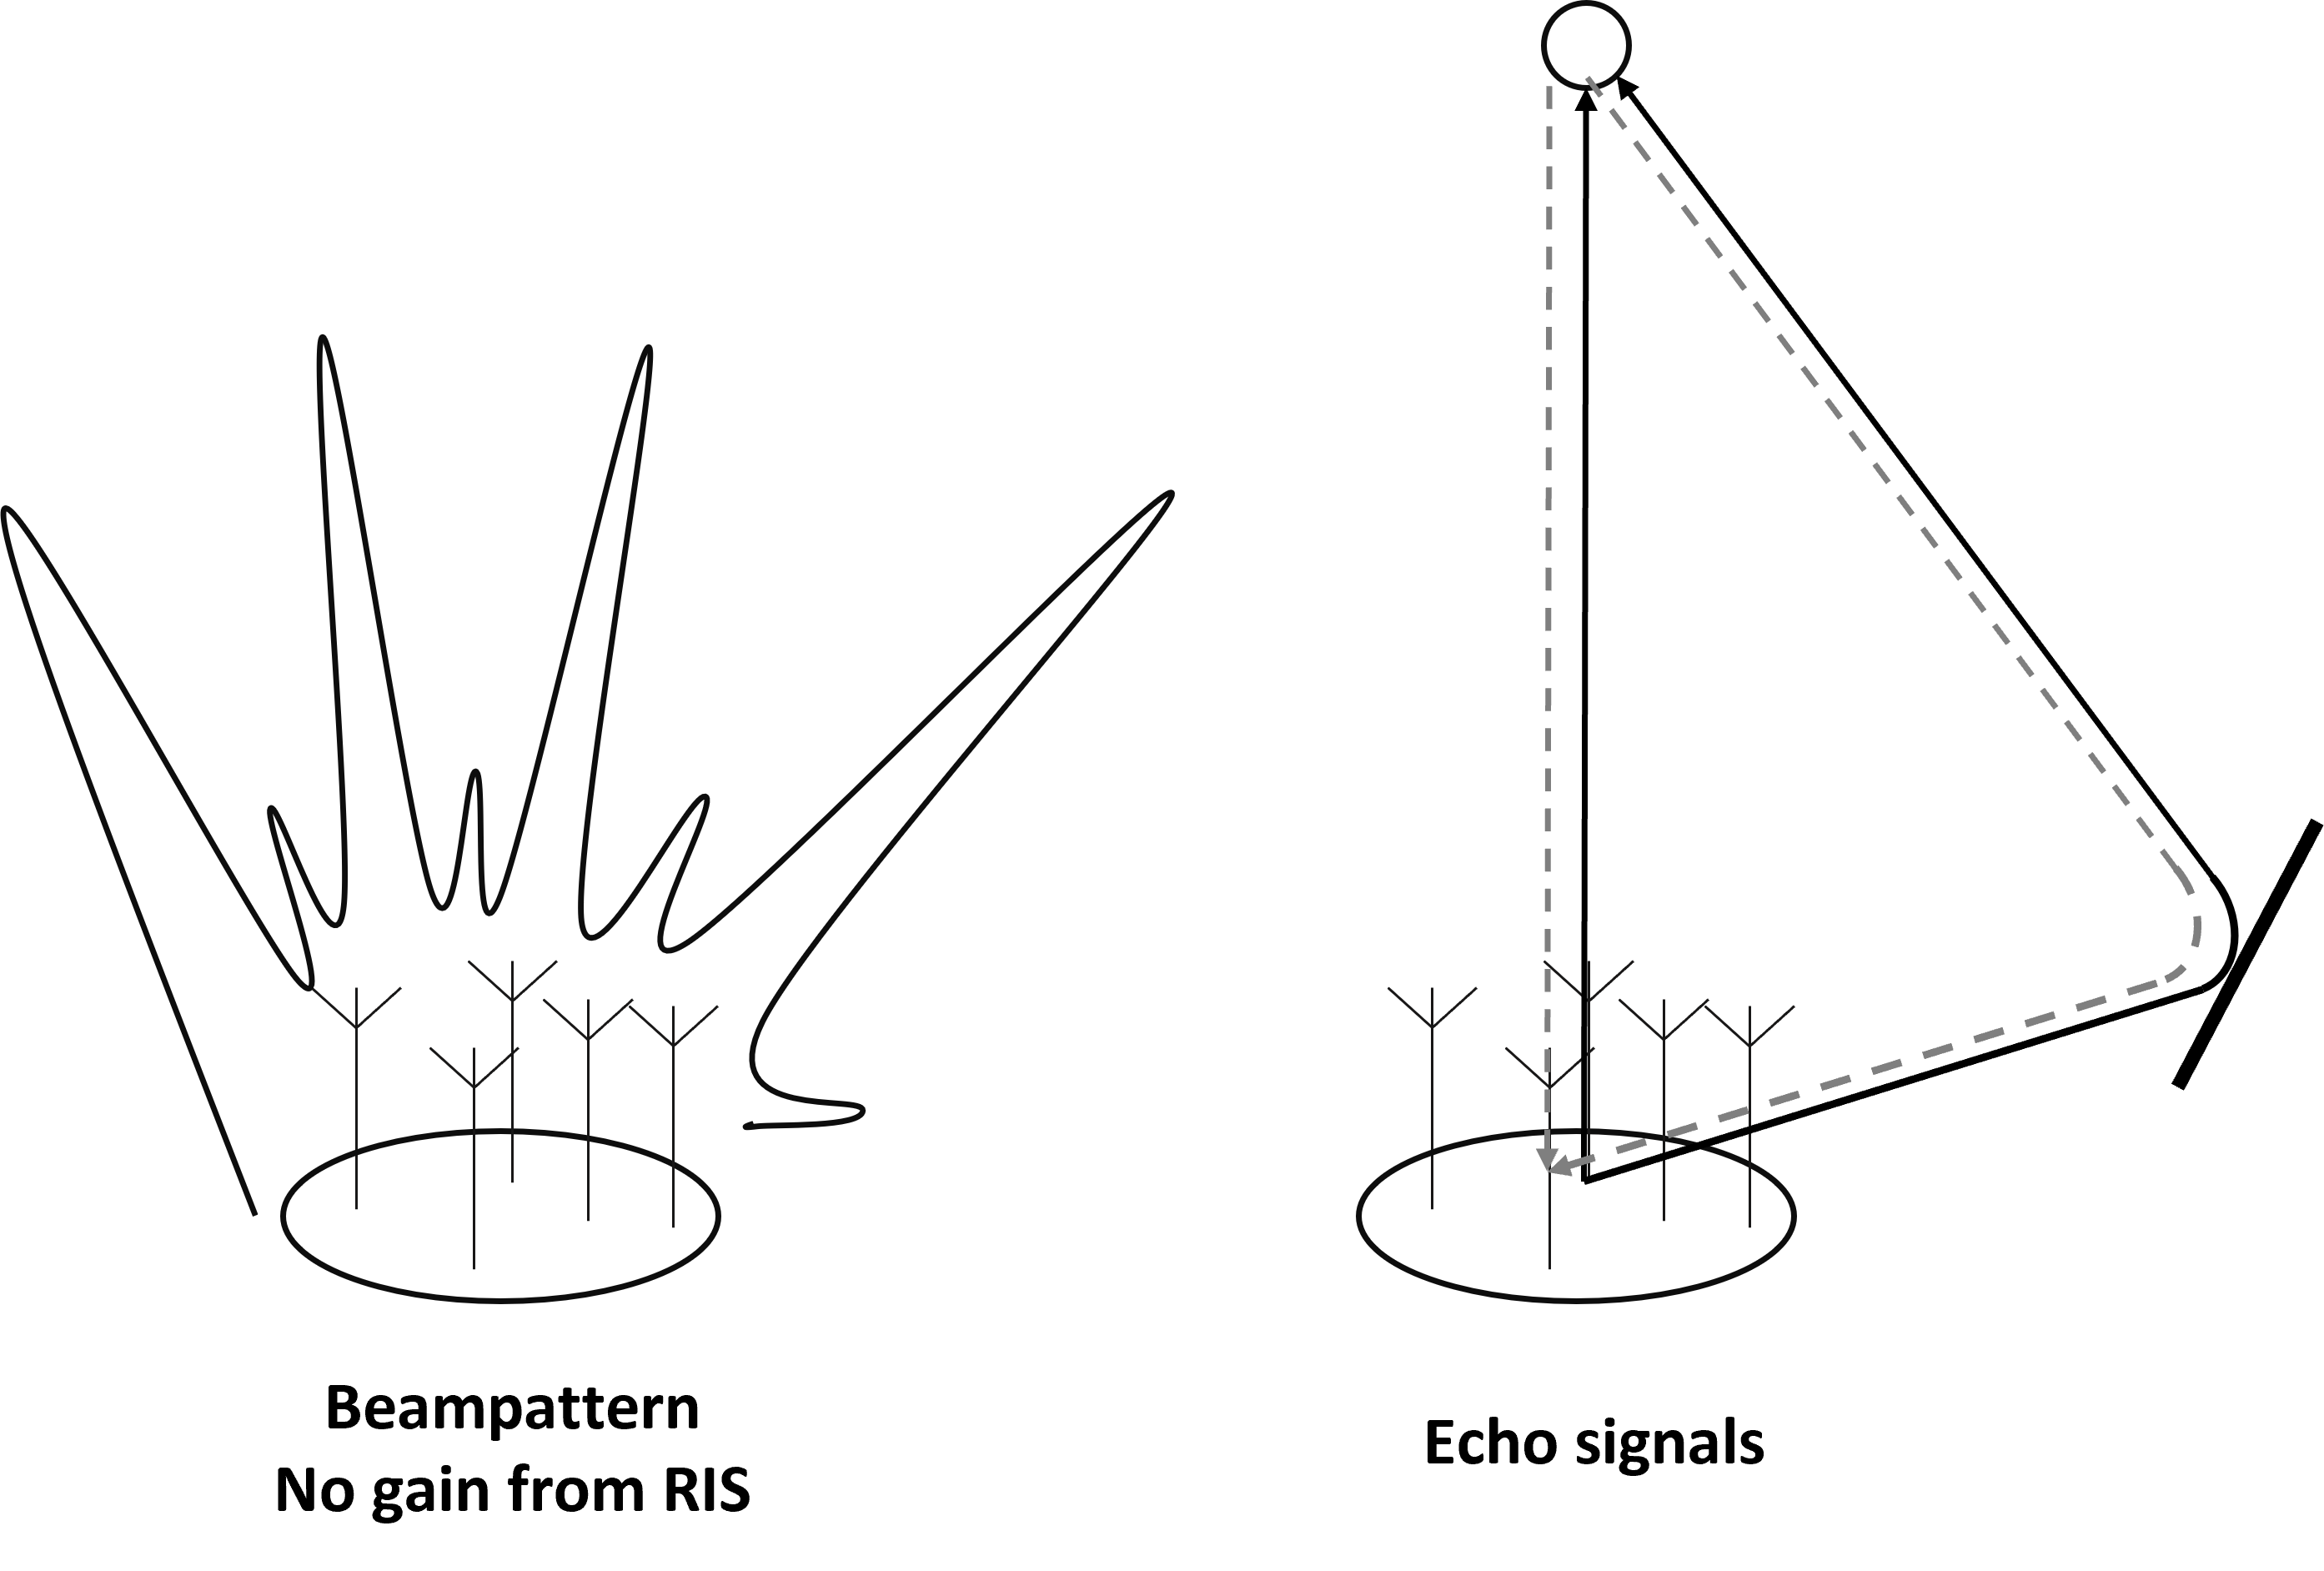
\includegraphics[width=0.6\linewidth]{./img/No-RIS_vs_RIS-aided.png}
    \end{figure}
\end{frame}

\begin{frame}
    \frametitle{On Dual-Functional Radar and Communications Design with Reconfigurable Intelligent Surface}
    \begin{block}{Conventional radar metrics}
        \begin{itemize}
        \small
        \item Detection: detection probability $P_D$ and false-alarm probability $P_{FA}$
        \item Estimation: mean square error
        \end{itemize}    
    \end{block}

    \begin{block}{Example}
        \small
        According to \cite{wang2020ris}, when the generalized likelihood ratio test under the
        Neyman-Pearson criterion is applied, the detection probability is given as
        \begin{equation}
            P_D = 1 - \mathfrak{F}_{\mathcal{X}_2^2(\rho)}\Big(\mathfrak{F}_{\mathcal{X}_2^2}^{-1}(1-P_{FA})\Big)
        \end{equation}
        If the radar signal is orthogonal, i.e., ${\bf R_r}=P_R{\bf I}_{N_t}$, and the echo signal is ${\bf y} = \beta{\bf Cr + z}$, 
        the parameter $\rho$ is
        \begin{equation}
            \rho = |\beta|^2 P_R {\rm Tr}\Big( {\bf CC}^H {\bf R}_{\bf z}^{-1} \Big) \geq {\rm SINR_{echo}}
        \end{equation}
    \end{block}
\end{frame}

\begin{frame}
    \frametitle{On Dual-Functional Radar and Communications Design with Reconfigurable Intelligent Surface}
    \begin{block}{Potential benefits of deep learning}
        \begin{itemize}
        \small
        \item Deep learning may catch up more information than conventional optimization method.
        % \item Deep learning may be helpful to reach the optimal metric without closed form.
        \item Deep learning algorithm may have lower complexity.
        \end{itemize}    
    \end{block}

    \begin{block}{A simple idea}
        \small
        Deep reinforcement learning: we can set the detection probability and WSR as reward, and the model will learn what is the optimal beamforming (actions) in different environments (states).
    \end{block}
\end{frame}
